% !TEX encoding = UTF-8
% !TEX program = pdflatex
% !TEX root = relazione.tex
% !TeX spellcheck = it_IT

% APPLICAZIONI REALI
\section{Applicazioni reali}
I grafici che seguono rappresentano i modelli tariffari scelti dalle varie piattaforme e mostrano il loro comportamento al variare del ``carico di lavoro''.
Nell'asse delle ascisse si trova, quindi, il numero di immagini (numero di chiamate con un'immagine ogni chiamata) processate al mese,
mentre nell'asse delle ordinate il corrispondente costo in dollari americani\footnote{Regione: West US}.
E' stata scelta questa valuta poiché tutti i servizi coprono il territorio americano (almeno in parte), mentre non è così per altre zone come l'europa;
una valuta come il dollaro, quindi, offre un metro di paragone fra tutti i servizi.

Il primo grafico in ~\ref{fig:grafico1} mostra le differenze di prezzo per riconoscimento di oggetti con un basso carico di immagini, includendo anche i piani gratuiti.
Come si può notare per poche immagini il sevizio offerto da Google non è conveniente, infatti offre gratuitamente solo 1000 chiamate al mese.
Bisogna però ricordare che l'IBM Visual Recognition offre mensilmente il maggior numero di chiamate ma il conteggio è giornaliero.
\begin{figure}[!h]
\begin{center}
	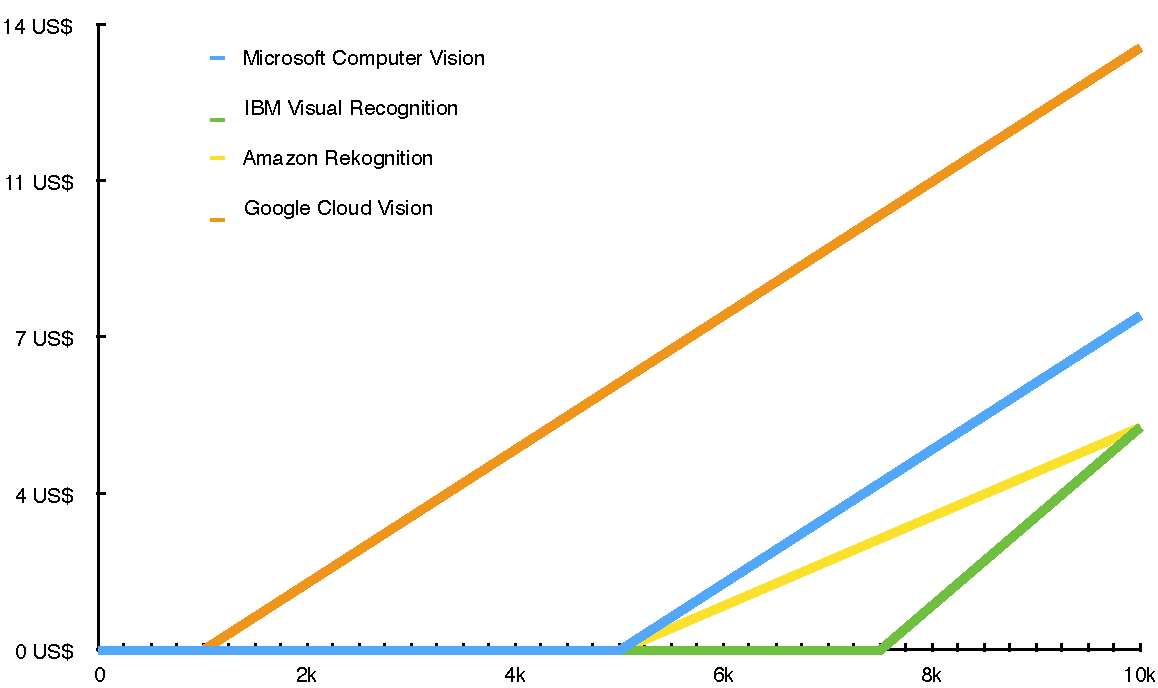
\includegraphics[scale=.4]{grafico1}
{\scriptsize
\caption{Riconoscimento oggetti con piano gratuito (da 0 a 10K di immagini)}
\label{fig:grafico1}}
\end{center}
\end{figure}
%
%
Rimuovendo il piano gratuito iniziale, le tariffe di Google e Microsoft si equivalgono mentre quella più conveniente sembra essere quello di Amazon,
come si evince dal grafico ~\ref{fig:grafico2}.
\begin{figure}[!h]
\begin{center}
	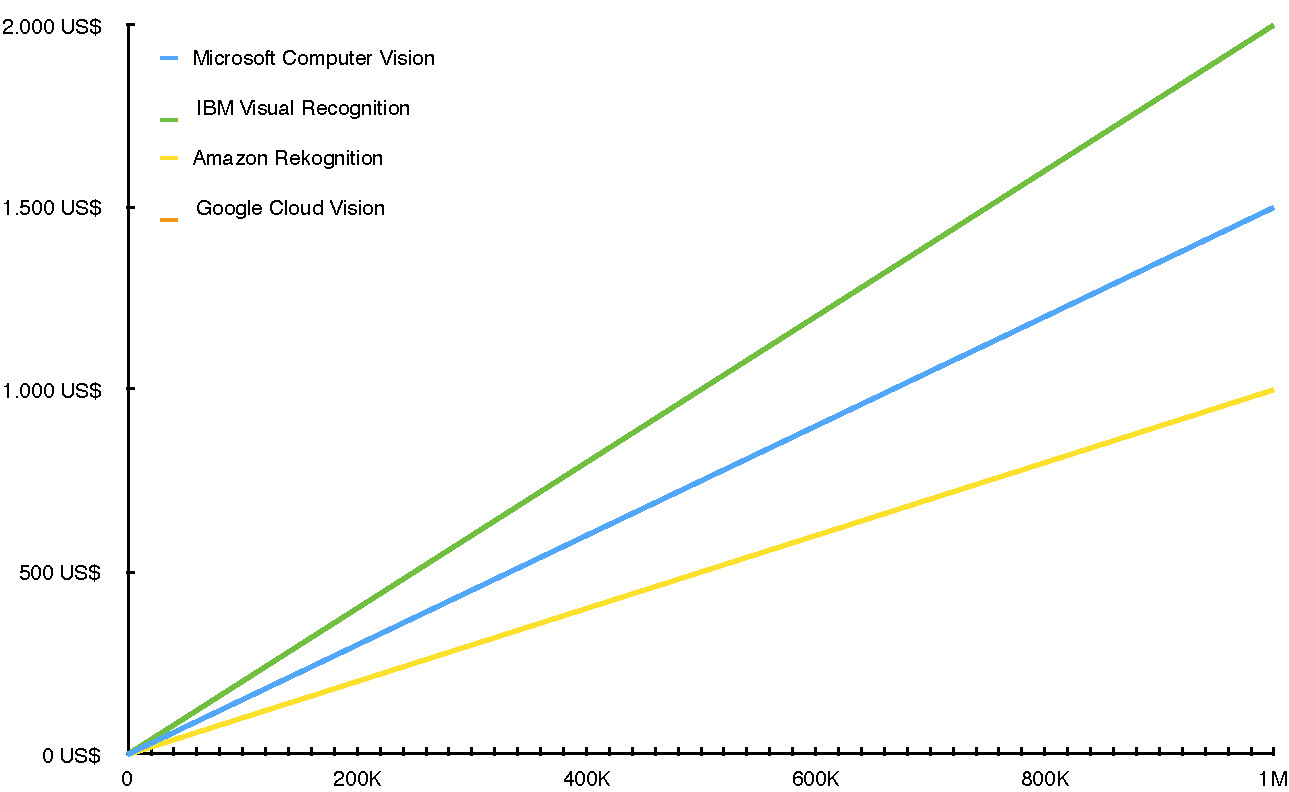
\includegraphics[scale=.4]{grafico2}
{\scriptsize \caption{Riconoscimento oggetti senza piano gratuito (da 0 a 1M di immagini)}
\label{fig:grafico2}}
\end{center}
\end{figure}
%
%
Gli ultimi due grafici, invece, mostrano le tariffe per scenari più reali, con carichi di lavoro dai 50 ai 150 milioni di immagini analizzate al mese.
Il primo ~\ref{fig:grafico3} rappresenta sempre il riconoscimento di oggetti mentre il secondo ~\ref{fig:grafico4} il riconoscimento dei volti.
Questo perché alcuni prevedono costi differenti per il riconoscimento di oggetti e di volti, come ad esempio IBM, dove il costo per la seconda è il doppio,
e Google, quando il numero di immagini al mese superano i cinque milioni.
\begin{figure}[!h]
\begin{center}
	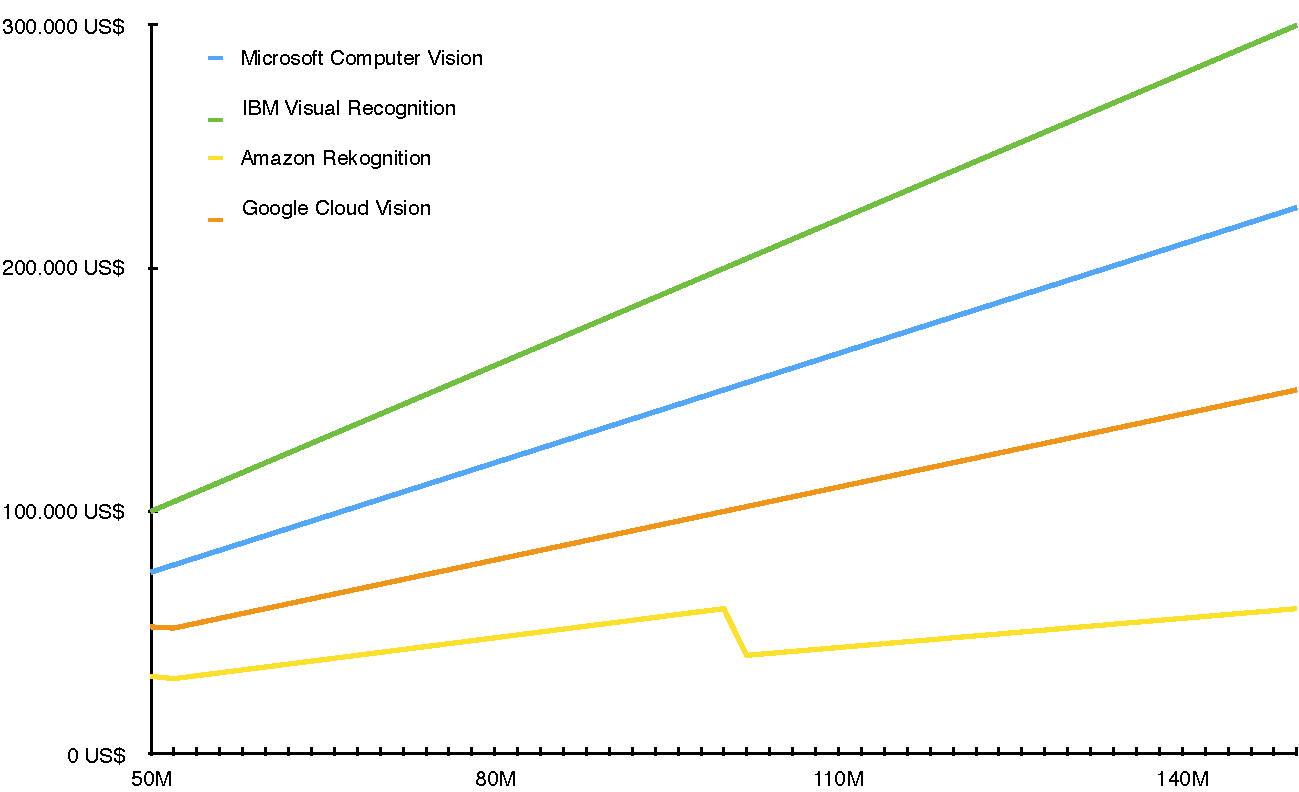
\includegraphics[scale=.4]{grafico3}
{\scriptsize \caption{Riconoscimento oggetti (da 50M a 150M di immagini)}
\label{fig:grafico3}}
\end{center}
\end{figure}
%
\begin{figure}[!h]
\begin{center}
	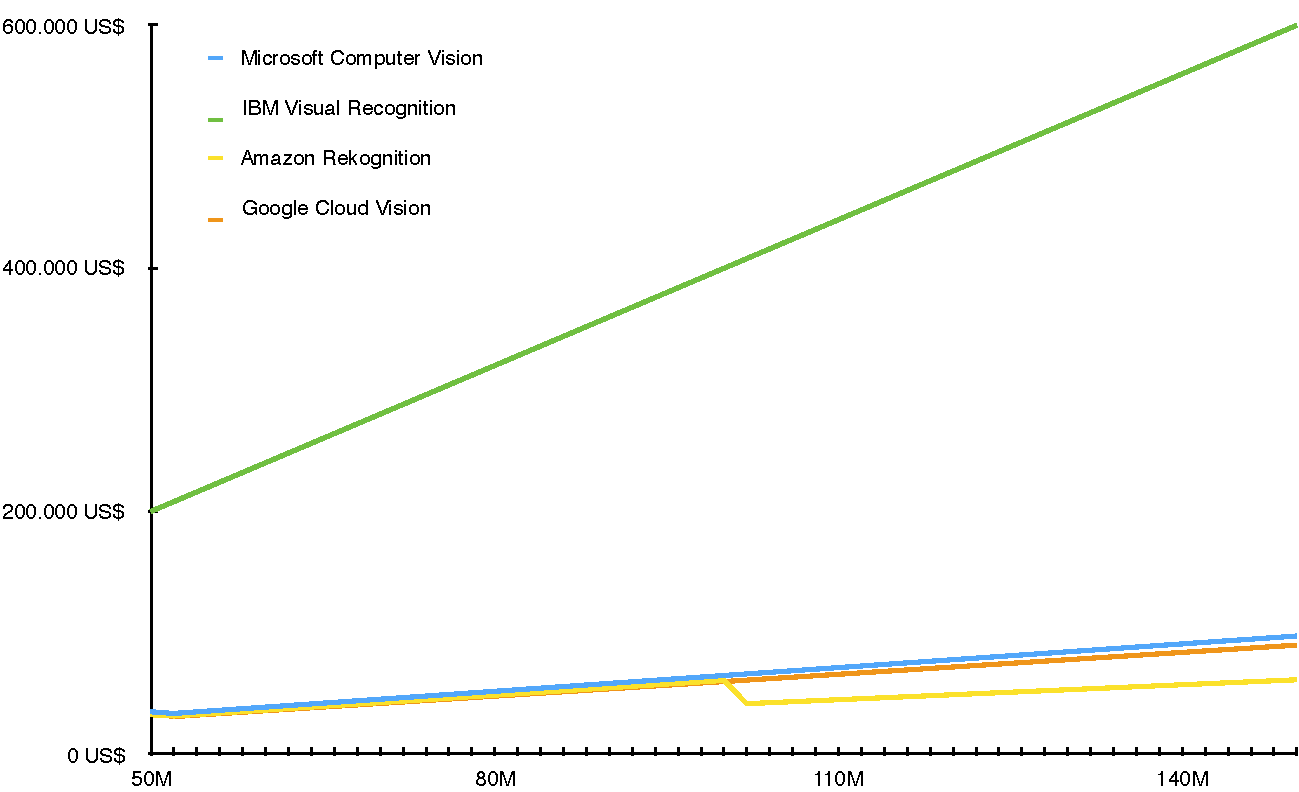
\includegraphics[scale=.4]{grafico4}
{\scriptsize \caption{Riconoscimento volti (da 50M a 150M di immagini)}
\label{fig:grafico4}}
\end{center}
\end{figure}
%
%

Ogni scenario è da considerarsi indipendente dagli altri e rappresenta la stima nel caso peggiore, basandosi su quando scritto nelle relative documentazioni;
per applicazioni concrete, infatti, contattando i fornitori di servizi si potrebbero ottenere tariffe più agevolate.
Inoltre, i costi sono stati calcolati tenendo conto solo delle API analizzate in precedenza, escludendo costi aggiungivi come ad esempio il costo dell'archiviazione.
%
%
